\documentclass [11pt,twoside]{article}
\usepackage[utf8]{inputenc}
\usepackage[T1]{fontenc}

%Page margins, header and footer positions
\usepackage{geometry}
 \geometry{
 a4paper,
 total={210mm,297mm},
 left=25mm,
 right=25mm,
 top=30mm,
 bottom=25mm,
 headsep=7mm}

\interfootnotelinepenalty=10000

%To display filling dots in the TOC for all entries
\usepackage[titles]{tocloft}
\renewcommand{\cftsecleader}{\cftdotfill{\cftdotsep}}

%Define new header and footer style
\usepackage{fancyhdr}

\pagestyle{fancy}
\fancyhf{}
\lhead{\color{Gray}{\small{Travlendar+ project by Daverio Fiorillo}}}
\lfoot{\textcolor{Gray}{\small{Copyright © 2017, Daverio Fiorillo – All rights reserved}}}
\rfoot{\textcolor{Gray}{\thepage}}
\renewcommand{\headrulewidth}{0pt}

%PACKAGES
\usepackage{wasysym}
\usepackage{pifont}
\usepackage{float}

\newcommand{\supported}{\ding{52}\xspace}
\newcommand{\unsupported}{\ding{55}\xspace}
\newcommand{\partsupported}{\textcolor{black!40}{\ding{52}}\xspace}
\newcommand{\lowsupported}{\textcolor{black!20}{\ding{52}}\xspace}
\newcommand{\unknowsupported}{\textbf{?}\xspace}

%Font: Times
\usepackage{times}
%Change monospaced font
\renewcommand{\ttdefault}{lmtt}

%tables
\usepackage{tabu}
\usepackage{tabularx}
\usepackage{ltablex}
\usepackage{longtable}
\usepackage{float} % To allow the use of H modifier in long tables

%landscape mode
\usepackage{pdflscape}
\usepackage{rotating}
\usepackage{caption}

%make landscape mode be sensitive to even and odd pages
%start
\def\myrotate{\ifodd\c@page\else-\fi 90}
\makeatletter
\global\let\orig@begin@landscape=\landscape%
\global\let\orig@end@landscape=\endlandscape%
\gdef\@true{1}
\gdef\@false{0}
\gdef\landscape{%
    \global\let\within@landscape=\@true%
    \orig@begin@landscape%
}%
\gdef\endlandscape{%
    \orig@end@landscape%
    \global\let\within@landscape=\@false%
}%
\@ifpackageloaded{pdflscape}{%
    \gdef\pdf@landscape@rotate{\PLS@Rotate}%
}{
    \gdef\pdf@landscape@rotate#1{}%
}
\let\latex@outputpage\@outputpage
\def\@outputpage{
    \ifx\within@landscape\@true%
        \if@twoside%
            \ifodd\c@page%
                \gdef\LS@rot{\setbox\@outputbox\vbox{%
                    \pdf@landscape@rotate{-90}%
                    \hbox{\rotatebox{90}{\hbox{\rotatebox{180}{\box\@outputbox}}}}}%
                }%
            \else%
                \gdef\LS@rot{\setbox\@outputbox\vbox{%
                    \pdf@landscape@rotate{+90}%
                    \hbox{\rotatebox{90}{\hbox{\rotatebox{0}{\box\@outputbox}}}}}%
                }%
            \fi%
        \else%
            \gdef\LS@rot{\setbox\@outputbox\vbox{%
                \pdf@landscape@rotate{+90}%
                \hbox{\rotatebox{90}{\hbox{\rotatebox{0}{\box\@outputbox}}}}}%
            }%
        \fi%
    \fi%
    \latex@outputpage%
}
\makeatother
%end

%graphics
\usepackage{graphicx}
\usepackage[dvipsnames, table]{xcolor}
%If you upload images from PC, you need to insert code for the path here (different for Windows and Unix OS)

%References
%\usepackage{xpatch}
%\usepackage[backend=biber, style=numeric, citestyle=numeric, sorting=none]{biblatex}
%\addbibresource{main.bib}

%Other
\usepackage{ifthen}
\usepackage{xspace}
\usepackage{enumitem}
\usepackage{amssymb}
\usepackage[pdftex, colorlinks]{hyperref}
\newcommand{\comment}[1]{{\color{Red}$\blacktriangleright$ Comment: #1 $\blacktriangleleft$}}


% Some utilities\ldots
\usepackage{soul}
\usepackage{tikz}

\usetikzlibrary{calc}
\usetikzlibrary{decorations.pathmorphing}


\makeatletter

\newcommand{\defhighlighter}[3][]{%
  \tikzset{every highlighter/.style={color=#2, fill opacity=#3, #1}}%
}

\defhighlighter{yellow}{.5}

\newcommand{\highlight@DoHighlight}{
  \fill [ decoration = {random steps, amplitude=1pt, segment length=15pt}
        , outer sep = -15pt, inner sep = 0pt, decorate
       , every highlighter, this highlighter ]
        ($(begin highlight)+(0,8pt)$) rectangle ($(end highlight)+(0,-3pt)$) ;
}

\newcommand{\highlight@BeginHighlight}{
  \coordinate (begin highlight) at (0,0) ;
}

\newcommand{\highlight@EndHighlight}{
  \coordinate (end highlight) at (0,0) ;
}

\newdimen\highlight@previous
\newdimen\highlight@current

\DeclareRobustCommand*\highlight[1][]{%
  \tikzset{this highlighter/.style={#1}}%
  \SOUL@setup
  %
  \def\SOUL@preamble{%
    \begin{tikzpicture}[overlay, remember picture]
      \highlight@BeginHighlight
      \highlight@EndHighlight
    \end{tikzpicture}%
  }%
  %
  \def\SOUL@postamble{%
    \begin{tikzpicture}[overlay, remember picture]
      \highlight@EndHighlight
      \highlight@DoHighlight
    \end{tikzpicture}%
  }%
  %
  \def\SOUL@everyhyphen{%
    \discretionary{%
      \SOUL@setkern\SOUL@hyphkern
      \SOUL@sethyphenchar
      \tikz[overlay, remember picture] \highlight@EndHighlight ;%
    }{%
    }{%
      \SOUL@setkern\SOUL@charkern
    }%
  }%
  %
  \def\SOUL@everyexhyphen##1{%
    \SOUL@setkern\SOUL@hyphkern
    \hbox{##1}%
    \discretionary{%
      \tikz[overlay, remember picture] \highlight@EndHighlight ;%
    }{%
    }{%
      \SOUL@setkern\SOUL@charkern
    }%
  }%
  %
  \def\SOUL@everysyllable{%
    \begin{tikzpicture}[overlay, remember picture]
      \path let \p0 = (begin highlight), \p1 = (0,0) in \pgfextra
        \global\highlight@previous=\y0
        \global\highlight@current =\y1
      \endpgfextra (0,0) ;
      \ifdim\highlight@current < \highlight@previous
        \highlight@DoHighlight
        \highlight@BeginHighlight
      \fi
    \end{tikzpicture}%
    \the\SOUL@syllable
    \tikz[overlay, remember picture] \highlight@EndHighlight ;%
  }%
  \SOUL@
}

\makeatother

% Common abbrev. are set as commands to ensure proper spacing after the dot
\RequirePackage{xspace}
\newcommand{\ie}{i.e.\@\xspace}
\newcommand{\aka}{a.k.a.\@\xspace}
\newcommand{\Ie}{I.e.\@\xspace}
\newcommand{\cf}{cf.\@\xspace}
\newcommand{\Cf}{Cf.\@\xspace}
\newcommand{\eg}{e.g.\@\xspace}
\newcommand{\Eg}{E.g.\@\xspace}
\newcommand{\etal}{et al.\@\xspace}
\newcommand{\etc}{etc.\@\xspace}
\newcommand{\wrt}{w.r.t.\@\xspace}
\newcommand{\Wrt}{W.r.t.\@\xspace}



\date{}


\begin{document}

%TITLE PAGE

\begin{titlepage}


%LOGO

{\begin{table}[t!]
\centering
\begin{tabu} to \textwidth { X[1.3,r,p] X[1.7,l,p] }
\textcolor{Blue}
{\textbf{\small{Travlendar+ project Daverio Pietro, Fiorillo Alessandro}}} & 
\includegraphics[scale=0.5]{Images/PolimiLogo}
\end{tabu}
\end{table}}~\\ [7cm]

%TITLE 

\begin{flushleft}

%Replace the text string with your title
{\textcolor{Blue}{\textbf{\Huge{Design Document}}}} \\ [1cm]

\end{flushleft}

\end{titlepage}

%Define deliverable specific info
%Replace cell contents where needed
\begin{table}[h!]
\begin{tabu} to \textwidth { X[0.3,r,p] X[0.7,l,p] }
\hline

\textbf{Deliverable:} & RASD\\
\textbf{Title:} & Design Document \\
\textbf{Authors:} & Daverio Pietro, Fiorillo Alessandro \\
\textbf{Version:} & 1.0 \\ 
\textbf{Date:} & 26-November-2018 \\
\textbf{Download page:} & https://github.com/FiorixF1/DaverioFiorillo \\
\textbf{Copyright:} & Copyright © 2018, Daverio, Fiorillo @ Politecnico di Milano \\
\hline
\end{tabu}
\end{table}




\setcounter{page}{2}


%------------------------------------------------------------------------------------------------------------------------------------------------
\newpage
\addcontentsline{toc}{section}{Table of Contents}
\tableofcontents
\newpage
\addcontentsline{toc}{section}{List of Figures}
\listoffigures
\addcontentsline{toc}{section}{List of Tables}
\listoftables

%------------------------------------------------------------------------------------------------------------------------------------------------
\clearpage
{\color{Blue}{\section{Introduction}}}
\label{sect:introduction}
\subsection{Purpose}
The following document is the Requirement Analysis and Specification Document (RASD) for the formalization and description of all the needed features, constraints and recommendations that will constitute the proposed system.

The paper will focus on the elicitation and analysis of all functional and nonfunctional requirements, also verified by automated logic verification software (Alloy Analyzer [MIT]) and supported by UML schemes and scenarios.
The provided document will also include a concise analysis of the environment and it tries to clarify all the interaction among system parts and external world.

The target audiences of this document are all the stakeholders involved in the development of the system and it can be used as contractual base for the project.


\subsection{Scope}

\subsubsection{System description}

The system that would be developed is a calendar-based application that provides support for planning of appointments, automating the travel arrangement process according to the user preferences.
The system will be able to plan travel routes choosing transport options among public and private means, including trains, trams, taxis, bicycles, bike and car sharing, owned automobile and others. Therefore, the system will provide a set of possible route options, trying to minimize travel times, route length, carbon footprint or number of changes.

Also, it will have to recollect travel informations on public transportations and travelling conditions from different external sources.
Beside, the application will give the possibility to users to register themselves, allowing them to access a series of extra features, including the possibility of setting personal preferences and backup personal agenda and routes.

User preferences include the possibility to set travel pauses, flexible launch (30 minute of travel pause between 11.30-14.30), enabling and disabling certains types of transportation means in a specific period of the day or anytime and in addition it will give the possibility to user to create profiles of preferences and link them to single appointments)
Finally, system should be capable to interacting with any type of external public transportation service, although it will focus on make available them in the city of Milan.

\subsubsection{World Phenomena}

Many public transport service companies offers the possibility to obtains informations on timetables, routes, stations and status of services in aggregate way providing public Application Public Interfaces (APIs). Thus it is guaranteed the theoretical possibility to make queries in any moment and get the latest valid informations on transports.

Others doesn’t offer the same possibilities; for instance Trenitalia hasn’t yet a public API, but there are different opensource projects that allow to fill the gap.

Moreover, a lot of web mapping services makes available public APIs too. In this case it is possible to get GPS location from an address or vice-versa, or update a portion of map and even process a route given a starting point and a destination.
All the required supported companies provide aforementioned services.

\subsubsection{Goals}
%what you write here is a comment that is not shown in the final text
\begin{itemize}
	\item[G1] Allow the user to add an appointment
	\subitem[G1.1] The user can add the date of the appointment through a calendar
	\subitem[G1.2] The user can select the location through a map
	\subitem[G1.3] The appointment must be processed by the system
	\item[G2] - Provide a route to the user for reaching the appointments
	\subitem[G2.1] The user must reach on time his/her appointments
	\subitem[G2.2] The user can choose the starting location and time of the route
	\subitem[G2.3] Generate routes according to the preferences of the user
	\subitem[G2.4] The application provides a route for each objective, minimizing each of these attributes: length, duration, number of changes, carbon footprint
	\subitem[G2.5] Always provide a route
	\subitem[G2.6] During strike days, public transportation must not be available
	\subitem[G2.7] Report unfavorable weather conditions
	\subitem[G2.8] Update unfavorable weather conditions
	\subitem[G2.9] The user can save one route among the shown ones
	\item[G3] Allow the user to sign up into the application
	\subitem[G3.1] The registration must allow the univocal recognition of the user
	\item[G4] Allow the user to log in
	\subitem[G4.1] The system allow the login through e-mail and password
	\subitem[G4.2] The application allow the login through telephone number
	\item[G5] Allow the user to add his own preferences
	\subitem[G5.1] The user must be logged
	\subitem[G5.2] The preferences are synchronized between the application and the database
	\subitem[G5.3] The user can chose the available transport means
	\subitem[G5.4] The user can add a priority to the means of transport
	\subitem[G5.5] The user can add the maximum length of routes on foot or by bicycle
	\subitem[G5.6] For each vehicle the user can choose a time slot of validity
	\subitem[G5.7] The user can set Flexible Lunch
	\subitem[G5.8] The user can add breaks for fixed moments of the day
	\subitem[G5.9] The user can add a private car or bicycle
	\subitem[G5.10] The user can organize his preferences in “Preferences Profiles"
	\item[G6] Allow the user to manage his account
	\subitem[G6.1] The user must be able to remove appointments and routes
	\subitem[G6.2] The user must be able to modify appointments and routes
	\subitem[G6.3] The user must be able to delete his account
	\item[G7] Allow the user to report events and disservices 
	\subitem[G7.1] The user can report strikes using the application
	\subitem[G7.2] The user can report faults, malfunctions and suggestions
\end{itemize}

\subsection{Definitions, Acronyms, Abbreviations}

\subsubsection{Definitions}
\begin{itemize}
	\item API(s) : Application Program Interface(s)
	\item RASD : Requirement Analysis Specification Document
	\item Appointment: location the user has to reach at a fixed date and time
	\item Route: journey between two appointments, it is composed by a series of paths
	\item Path: part of a route traversed with a specific mean of transport
\end{itemize}


\subsubsection{Acronyms}
\begin{itemize}
	\item UI: User Interface
\end{itemize}

\subsubsection{Abbreviations}
\begin{itemize}
	\item MA (Mobile Application): part of the system
	\item PT: Public Transportation
\end{itemize}

\subsection{Revision history}




\subsection{References}


\begin{itemize}
	\item Specification Document assigned: \texttt{“Mandatory\_Project\_Assignments.pdf”}
	\item Software Requirements Specification Guidelines : IEEE 830-1998
	\item Alloy Website: \url{http://alloy.mit.edu/alloy/}
\end{itemize}

\subsection{Document Structure}

The document is composed of six different parts.

\begin{enumerate}
	
	\item The introduction has the objective to support the reader into the reading of the document providing a brief description of the problem and the actual technological landscape description. It also include a list of definition, abbreviations and acronyms commonly employed through the rest of the document.
	\item The second part offers an overall description of the system, then focused on the boundaries that divide the system from world, especially inspecting all interactions on shared phenomena. In addition, it is provided a short description of users. FInally, it is listed and described a set of core functionalities that will be supported and assumptions.
	\item The third part provides a more complex and detailed description of functionalities, also in terms of requirement. This part is addressed specifically to development team
	\item This section provides an Alloy model for verification of goals through a formal analysis of requirements and domain assumption. This is beneficial in assuring the consistency of the model. It also provide a representation of the world and system.
	\item The fifth part provides the effort spent in term of time involved into the project by the authors.
	In the last part, there are references to external sources.
	
\end{enumerate}



%------------------------------------------------------------------------------------------------------------------------------------------------
\clearpage
{\color{Blue}{\section{Architectural Design}}}
\label{sect:architecture}
%Architectural Design section

\subsection{Overview}
% High level components and their interactions

This chapter will illustrate the architecture of the system with its logical and physical components and how they interact to reach the goals. The sections of this chapter are:
\begin{itemize}
	\item \emph{High level components and their interactions}: it provides a general idea about the physical components of the system
	\item \emph{Component view}: it shows the strctures of the logical components and how they communicate with each other
	\item \emph{Deployment view}: it describes the physical structure of the system and shows where each component will be deployed. It will also present the possible technologies that will be used for the implementation.
	\item \emph{Runtime view}: it presents how the components communicate with each other inside the most important scenarios that will be handled by the application
	\item \emph{Component interfaces}: it describes the interfaces between the components of the system
	\item \emph{Selected architectural styles and patterns}: it explains the patterns and architectural paradigms that have been used in some aspects of the architectural desig
	\item \emph{Other design decisions}: it presents further design choices that are worth mentioning
\end{itemize}

\subsection{High level components and their interactions}

The high level structure of the system follows a three-tier architecture. The client side is developed as a website and a mobile application, which are the interface of the user to the services of the system. The server contains all the business logic and is divided into several components. Each of them has a specific role and acts as an interface for other components and uses the interface provided by other components. Some other services participate in the functioning of the system but are outside the server: these are the external services, used for calculating routes, solve addresses into GPS coordinates and checking the weather conditions. Other external components let the application send push notification and SMS to the phone of a user. Finally, the last tier is realized by the database server, which is external to the main server hosting the business logic.

\newpage

\subsection{Component view}

\begin{figure}
\centering
\includegraphics[width=\textwidth]{{"Images/Architecture - Component View"}.png}
\caption{\label{fig:metamodel2}Component diagram of the system}
\end{figure}

\begin{itemize}
	\item \emph{Web Application}: client side component for the application via web browser
	\item \emph{Mobile Application}: client side component for the application via mobile device
	\item \emph{SessionManager}: handles login, sign up and general account functionalities
	\item \emph{NotificationManager}: handles notifications for weather forecast, incoming routes and account recovering by phone number
	\item \emph{CalendarManager}: handles the calendar and its appointments
	\item \emph{RouteManager}: handles routes and their generation
	\item \emph{ReportManager}: handles functionalities for reporting issues and suggestions
	\item \emph{PreferenceManager}: handles the settings of the user, in particular for route computation
	\item \emph{SMS Gateway}: service for sending SMS
	\item \emph{Push Gateway}: service for sending push notifications
	\item \emph{Weather Services}: external API for weather forecast
	\item \emph{Map Services}: external API for maps
	\item \emph{Route Services}: external API for routing
	\item \emph{Database}: the database of the system
\end{itemize}

The SessionManager exposes an interface for client users and it is a sort of dispatcher of the requests, since the available functionalities are different for registered users and normal users.

All the functionalities of the system are divided among the corresponding manager. The need some external services for fulfilling their task, which are represented as external components. Other external components are the Push Gateway and the SMS Gateway, which are not mandatory but provide a better user experience.

\subsection{Deployment view}

The architecture is divided in the following tiers:
\begin{itemize}
	\item \textbf{Client tier}: it is the interface of the application to the user, executable as a website on a browser or a graphical interface on a mobile device. The website is realized with the classical tools HTML5 and CSS, while the mobile application is available on Android and iOS operating systems.
	\item \textbf{Web tier}: it contains the web server which receives the HTTP requests from the web client and answers with HTML pages generated by a script engine. It can be implemented by the Tomcat web server and the JSP containers of Java EE.
	\item \textbf{Application tier}: it contains the core of the application with all the running components. It can be implemented using the Glassfish application server and the logic is contained in stateless Java beans. The communication with database happens with the JPA interface.
	\item \textbf{Database tier}: it contains the DBMS with the persistent data. It is accessible only by the application tier. A possible implementation will use the MySQL database.
\end{itemize}

\clearpage

\begin{figure}
\centering
\includegraphics[width=\textwidth]{{"Images/Architecture - Deployment View"}.png}
\caption{\label{fig:metamodel2}Deployment diagram of the proposed implementation}
\end{figure}

\subsection{Runtime view}
%Sequence diagrams to describe the way components interact to accomplish each task from use cases

The following sequence diagrams show the interaction between the components of the system while fulfilling the main features of the application. The features have been chosen in such a way that every component appears at least once in any sequence diagram, so that every component can be observed while operating in a scenario.

\begin{figure}
\centering
\includegraphics[width=\textwidth]{{"Images/Architecture - Runtime View - Log in"}.png}
\caption{\label{fig:metamodel2}User login}
\end{figure}

\begin{figure}
\centering
\includegraphics[width=\textwidth]{{"Images/Architecture - Runtime View - Add appointment"}.png}
\caption{\label{fig:metamodel2}Add an appointment}
\end{figure}

\begin{figure}
\centering
\includegraphics[width=\textwidth]{{"Images/Architecture - Runtime View - Add route"}.png}
\caption{\label{fig:metamodel2}Add a route}
\end{figure}

\begin{figure}
\centering
\includegraphics[width=\textwidth]{{"Images/Architecture - Runtime View - Notification"}.png}
\caption{\label{fig:metamodel2}Send a notification (push or SMS)}
\end{figure}

\clearpage

\subsection{Component interfaces}

As shown in the component diagram, all components are interconnected. Here follows an explanation of the services offered and used by each component.

\begin{itemize}
	\item The \emph{SessionManager} offers an interface to the client tier. It gives the possibility for a user to login or sign up, using also the phone number. All the requests made by a user pass through this interface, checking if a user has the right to make that request and then forwarding it to the correct component.
	\item The \emph{NotificationManager} offers methods to send push notifications and SMS messages. These methods are used by the SessionManager for allowing a user to login with a phone number, and by the CalendarManager to warn a user that a registered appointment or route is going to begin. This component relies on external services for delivering the messages.
	\item The \emph{CalendarManager} is the container of the methods to handle the calendar and the appointments. It uses the interfaces of RouteManager and ReportManager for managing routes and reporting issues. Also map services are required when solving the addresses of the appointments.
	\item The \emph{RouteManager} has the task to create, calculate and manipulate routes according to the needs of a user. It needs the external map and routing services and uses the PreferenceManager to get the necessary constraints while building a route.
	\item The \emph{PreferenceManager} allows to create and manage the preference profiles of a user.
	\item The \emph{ReportManager} allows to register issues, reports and suggestions written by users.
\end{itemize}

\subsection{Selected architectural styles and patterns}

As shown previously, the architecture is basically divided into three tiers where:

\begin{itemize}
	\item The \textbf{client tier} is a graphical interface for the user with little data manipulation
	\item The \textbf{server tier} contains most of the business logic
	\item The \textbf{database tier} stores all the required data
\end{itemize}

With this perspective, the most suitable design patterns are the following:

\begin{itemize}
	\item \textbf{Facade pattern}: a single interface is shown outside the server to the clients. The requests will be then forwarded to the necessary manager.
	\item \textbf{Proxy pattern}: the SessionManager acts not only as a request dispatcher, but also as a request filter, to distinguish the rights of a normal user from those of a registered user.
	\item \textbf{Adapter pattern}: the application makes high use of external services, which are unlikely to not change, be expanded or be replaced by other services. This is why the internal components of the server won’t communicate directly with the services, but will use the methods offered by some adapter classes.
	\item \textbf{Observer pattern}: for allowing push notifications, it is reasonable to use this simple and robust pattern.
\end{itemize}

\subsection{Other design decisions}

In Section 2.1.3 of RASD a list of software interfaces are provided. Those will be the external services that will be used inside the application for routing and weather forecast. For map services, an open API will be used.

%------------------------------------------------------------------------------------------------------------------------------------------------
\clearpage
{\color{Blue}{\section{Algorithm Design}}}
\label{sect:algorithms}
Organize this section according to the rules defined in the project description. 


%------------------------------------------------------------------------------------------------------------------------------------------------
\clearpage
{\color{Blue}{\section{User Interface Design}}}
\label{sect:interface}
\subsection{Mock ups}


The following mock-ups give an idea of how the mobile user interface will be structured. The software used for realizing these mock-ups is Pencil, which doesn't produce very nice looking interfaces, but it is helpful for creating a structure that will be followed when realizing the real user interface.

\begin{figure}[h]
\centering
\includegraphics[scale=0.5]{{"Images/UI - Login"}.png}
\caption{\label{fig:metamodel2}Login screen}
\end{figure}

\begin{figure}
\centering
\includegraphics[scale=0.5]{{"Images/UI - Signup"}.png}
\caption{\label{fig:metamodel2}Sigup screen}
\end{figure}

\begin{figure}
\centering
\includegraphics[scale=0.5]{{"Images/UI - Home"}.png}
\caption{\label{fig:metamodel2}Home screen with calendar}
\end{figure}

\begin{figure}
\centering
\includegraphics[scale=0.5]{{"Images/UI - Add appointment"}.png}
\caption{\label{fig:metamodel2}Add an appointment}
\end{figure}

\begin{figure}
\centering
\includegraphics[scale=0.5]{{"Images/UI - Add route"}.png}
\caption{\label{fig:metamodel2}Add a route}
\end{figure}

\begin{figure}
\centering
\includegraphics[scale=0.5]{{"Images/UI - Preferences"}.png}
\caption{\label{fig:metamodel2}Set preferences}
\end{figure}

\begin{figure}
\centering
\includegraphics[scale=0.5]{{"Images/UI - Select route"}.png}
\caption{\label{fig:metamodel2}Select a route}
\end{figure}

\clearpage

\subsection{UX diagram}

The following UX diagram shows how a user of the application would navigate through the different screens while using the available features. Each screen is represented as a class with stereotype «screen» and contains the possible functionalities, while the classes with stereotype «input form» contains attributes that the user must provide inside a specific screen. The diagram has been created following the structure of the mockups in the previous paragraph.

\begin{sidewaysfigure}
\centering
\includegraphics[width=\textwidth]{{"Images/UI - UX Diagram"}.png}
\caption{\label{fig:metamodel2}UX Diagram}
\end{sidewaysfigure}

%------------------------------------------------------------------------------------------------------------------------------------------------
\clearpage
{\color{Blue}{\section{Requirements Traceability}}}
\label{sect:traceability}
 


%------------------------------------------------------------------------------------------------------------------------------------------------
\clearpage
{\color{Blue}{\section{Implementation, Integration and Test Plan}}}
\label{sect:implementation}
%Implementation, Integration and Test Plan

\subsection{Integration conditions}

\subsubsection{Entry Criteria}

Integration and testing processes should be performed on each single unit as soon as the component has been fully developed. In addition, integration of different components should be perform only if all these criteria are satisfied:

\begin{itemize}
	\item RASD and DD documents can be considered "stable", therefore it isn't expected any other modification of requirements or structure of the system, furthermore both deliverables ought to be distributed to all developer team involved in the project.
	\item There are same dependencies in integration and testing plan that have to be satisfied in order to guarantee the possibility to perform useful cross-components tests on functionalities, because of intrinsic bounds of the architecture.
	\begin{enumerate}
		\item \textit{Map Services} and \textit{Route Services} for \textit{RouteManager}
		\item \textit{SMS Gateway} and \textit{Push Gateway} for \textit{NotificationManager}
		\item \textit{Map Services} for \textit{MA} and \textit{WebUI}
		\item \textit{DBMS} for \textit{CalendarManager}, \textit{ReportManager} and \textit{PreferenceManager}
		\end{enumerate}
\end{itemize}

\subsubsection{Elements to be integrated}

It is possible to distinguish three different categories of components, basing the grouping on set of functionalities covered, their interaction and integration dependencies.
\vspace{0.3cm}
\begin{itemize}
	\item \textbf{FrontEnd components}: set of units involved in the management of interactions between the system and user. Its modules are distributed among web and client tiers.
	\begin{enumerate}
		\item \textit{Mobile Application}
		\item \textit{Web Application}
		\item \textit{SessionManager}
	\end{enumerate}
	\item \textbf{BackEnd components}: units that provides the business logic for all system's features. Entirely located on application tier.
	\begin{enumerate}
		\item \textit{SessionManager}
		\item \textit{CalendarManager}
		\item \textit{RouteManager}
		\item \textit{PreferenceManager}
		\item \textit{NotificationManager}
	\end{enumerate}
	\item \textbf{Services components}: atomic components, without any dependency, each one provides a single basic functionality to the system. They are mainly located on the application tier.
	\begin{enumerate}
		\item \textit{DBMS}
		\item \textit{Route Services}
		\item \textit{Map Services}
		\item \textit{WeatherServices}
		\item \textit{Push Gateway}
		\item \textit{SMS Gateway}
	\end{enumerate}
\end{itemize}
\subsection{Implementation, Integration Strategy}

Given the foretold component categorization, it is possible to easily set up a bottom up strategy for the integration of implemented components. This plan aims to reduce the whole testing effort needed to deploy complex drivers and stubs employed in the integration process.

The following integration plan will give higher priority to implementation, integration and unit test to components that doesn't rely on undeveloped ones.
According to that scheme, the first developing iteration will focus on \textit{services components}, followed by units with less unsatisfied dependencies.

It is also possible to parallelize large part of the development process working on parallel branches of the integration sequence diagram, smoothing the entire development process, without modifications to the integration and testing strategy.

Actually, the development of some component parts can be developed separately and asynchronously respect the unit itself. This practise is encouraged in order to offer the possibility to testing vertically some core functionalities of the system before the end of development. Further details on thread testing strategy in \ref{testplan}.

It is provided a list of functionalities and unit parts that can be implemented and integrated interdependently for testing purpose:
\begin{itemize}
	\item \textbf{\textit{Registration and Login}}
	\subitem \textit{Web Application}: UI with login/registration functionalities
	\subitem \textit{Mobile Application}: UI with login/registration functionalities
	\subitem \textit{SessionManager}: login/registration and client communication implemented
	\subitem \textit{DBMS}: implemented
	
	\item \textbf{\textit{Appointment management}} (add/remove/modify an appointment) without routes definition
	\subitem \textit{Web Application}: UI with appointment management functionalities
	\subitem \textit{Mobile Application}: UI with appointment management functionalities
	\subitem \textit{SessionManager}: appointment management and client communication implemented
	\subitem \textit{CalendarManager}: appointment management implemented
	\subitem \textit{DBMS}: implemented
	
	\item \textbf{\textit{Preference management}} (add/remove/modify preferences), requires \textit{Registration and Login}
	\subitem \textit{Web Application}: UI with preference management functionalities
	\subitem \textit{Mobile Application}: UI with preference management functionalities
	\subitem \textit{SessionManager}: preference management and implemented
	\subitem \textit{PreferenceManager}: preference management implemented
	\subitem \textit{DBMS}: implemented
\end{itemize}

\subsubsection{Integration sequence}

Directed arc from component-A to component-B is intended as a dependency of component-B on functionalities offered by component-A.
The implementation, integration and testing scheme starts from the bottom with first to be developed units, and propagates to the top, stepping forward only if all dependencies are satisfied.

\begin{sidewaysfigure}
	\centering
	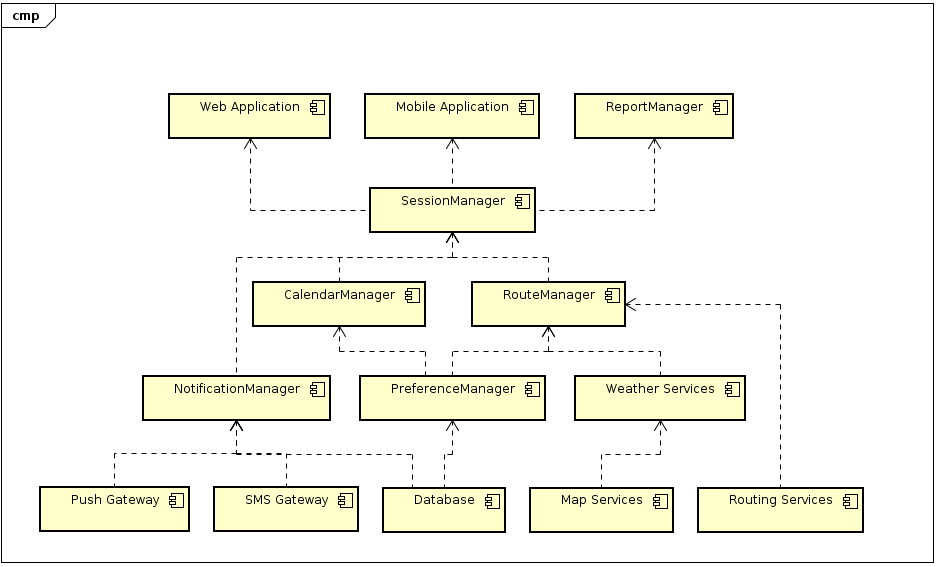
\includegraphics{Images/IntegrationDiagram.png}
	\caption{\label{fig:integration} Bottom-Up integration and testing components diagram. }
\end{sidewaysfigure}

\clearpage %Fix pictures position before this and newpage command

\subsubsection{Test Strategy}
\label{testplan}

While the system is suppose to be developed mainly through a bottom-up strategy, testing would be performed on each component as soon it is developed. Furthermore, it will also be verified the integration among component and all his dependency through specific integration tests. 

For some functionalities it is suggested to make exception because, for these ones, it is possible:

\begin{itemize}
	\item to split the deployment effort required by larger components, increasing atomicity of architecture unit in subcomponents;
	\item to anticipate the verification of some core features, that the system provides to user, far before the system test;
	\item to parallelize the development of an otherwise monolithic part of the implementation plan (particularly The \textit{SessionManager} module)
\end{itemize}

Functionalities should be verified as soon as needed components are available (list of goals and involved components is provide in \textit{Requirement Traceability} section \ref{sect:traceability}).

%------------------------------------------------------------------------------------------------------------------------------------------------
\clearpage
{\color{Blue}{\section{Effort Spent}}}
\label{sect:effort}

\subsection{Fiorillo}

\begin{tabular}{|c|c|}
	\hline
8/10/2017	& 45m \\ 
	\hline 
11/10/2017	& 45m \\ 
	\hline 
12/10/2017	& 1h20m \\ 
	\hline 
13/10/2017	& 1h \\ 
	\hline 
15/10/2017	& 2h \\ 
	\hline 
23/10/2017	& 1h15m \\ 
	\hline 
24/10/2017	& 30m \\ 
	\hline 
26/10/2017	& 2h15m \\ 
	\hline 
28/10/2017	& 30m \\ 
	\hline
29/10/2017	& 3h \\ 
	\hline
TOT			& 13h20m \\

\end{tabular} 

\subsection{Daverio}

\begin{tabular}{|c|c|}
	\hline
	2/10/2017	& 30m \\ 
	\hline 
	4/10/2017	& 40m \\ 
	\hline 
	7/10/2017	& 30m \\ 
	\hline 
	10/10/2017	& 2h20m \\ 
	\hline 
	14/10/2017	& 1h40m \\ 
	\hline 
	18/10/2017	& 3h \\ 
	\hline 
	20/10/2017	& 45m \\ 
	\hline 
	21/10/2017	& 1h20m \\ 
	\hline 
	25/10/2017	& 1h45m \\ 
	\hline 
	27/10/2017	& 7h45m \\ 
	\hline 
	28/10/2017	& 9h30m \\ 
	\hline
	29/10/2017	& 16h45m \\ 
	\hline
	TOT			& 47h30m \\

\end{tabular}


%------------------------------------------------------------------------------------------------------------------------------------------------
\clearpage
\addcontentsline{toc}{section}{References}
\bibliographystyle{plain}
\bibliography{main}
%------------------------------------------------------------------------------------------------------------------------------------------------




\end{document}
